\documentclass{article}
\usepackage{graphicx,amsmath,amssymb}
\usepackage{titling}
\usepackage{setspace}
\usepackage{fancyhdr}
\usepackage{enumerate}
\usepackage{bm}
\usepackage{textcomp, color}

\graphicspath{{../figs/}}

\renewcommand{\labelenumi}{\alph{enumi})}
\newcommand{\note}{\textcolor{black}}

\topmargin = -0.5in \textwidth=6.5in \textheight=8.8in

\oddsidemargin = 0in \evensidemargin = 0in

\title{Supporting Information}
\author{Julie Chang, Gordon Wetzstein}

\begin{document}
\maketitle

This document contains supporting information for the primary paper ``Single-shot speckle correlation fluorescence microscopy in thick scattering tissue with image reconstruction priors". We include additional simulations on the MNIST dataset, a 2D toy examples, and complete simulation results (non-averaged). 

%%%%%%%%%%%%%%%%%%%%%%%%%%%%%%%%%%%%%%%

\section{Single layer simulations on MNIST dataset}



\begin{figure}[h]
\centering
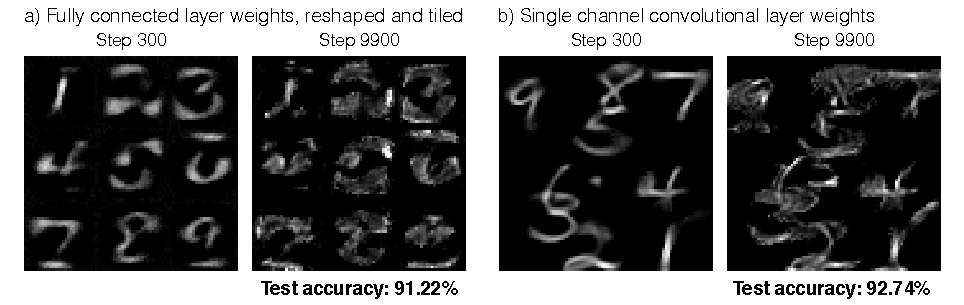
\includegraphics[width=\linewidth]{mnist.pdf}
\caption{MNIST simulation.}
\label{fig:mnist}
\end{figure}

%%%%%%%%%%%%%%%%%%%%%%%%%%%%%%%%%%%%%%%

\section{Effect of negative weights}

\begin{figure}[h]
\centering
\includegraphics[width=\linewidth]{supp_2d.pdf}
\caption{2D simulation.}
\label{fig:2d}
\end{figure}


%%%%%%%%%%%%%%%%%%%%%%%%%%%%%%%%%%%%%%%
\section{Local minima in end-to-end optimization}

\begin{figure}[h]
\centering
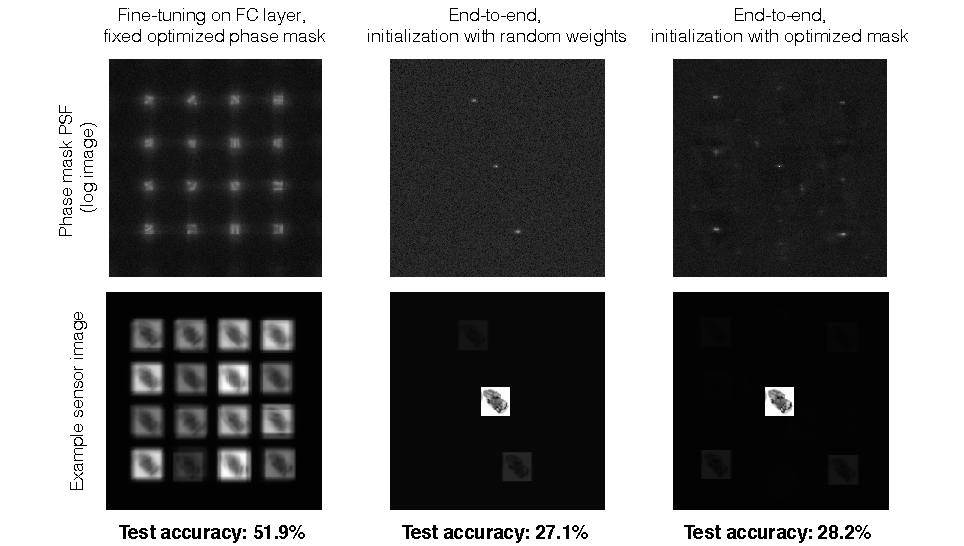
\includegraphics[width=\linewidth]{hybrid_e2e.pdf}
\caption{Comparing first layers of multi-step and end-to-end optimization.}
\label{fig:end2end}
\end{figure}

%%%%%%%%%%%%%%%%%%%%%%%%%%%%%%%%%%%%%%%

\section{Full simulation results}

\subsection{Optical correlator}

\subsection{Hybrid optoelectronic ONN}




%%%%%%%%%%%%%%%%%%%%%%%%%%%%%%%%%%%%%%%
\pagebreak
\begin{thebibliography}{00}

\bibitem{judkewitz2015} B. Judkewitz, R. Horstmeyer, I. Vellekoop, I. Papadopoulos, and C. Yang, Nat. Phys. \textbf{11}, 684--689 (2015). 


\end{thebibliography}

\end{document}
